\documentclass{article}

%%% Fill details here (in the second brackets)
\newcommand{\name}{Chris Bonney}     % Your name (First Last)
\newcommand{\wustlkey}{crbonney}             % Your WUSTL Key
%%%



%%%%%%%%%%%%%%%%%%%%%% Formatting Stuff %%%%%%%%%%%%%%%%%%%%%%%%%%%
\usepackage{times}
\usepackage[T1]{fontenc}

\setlength{\parskip}{1em}\setlength{\parindent}{0pt}
\linespread{1.25}
\usepackage[margin=0.7in,top=1in]{geometry}\usepackage{fancyhdr}
\pagestyle{fancy}\lhead{\bf \name}\rhead{\bf \wustlkey}\cfoot{\thepage}
\newcommand{\info}{\clearpage \subsection*{Information}}
\newcommand{\solution}[1]{\clearpage \subsection*{Solution #1}}
\newcommand{\spart}[1]{\paragraph{(#1)}}
%%%%%%%%%%%%%%%%%%%%%%%%%%%%%%%%%%%%%%%%%%%%%%%%%%%%%%%%%%%%%%%%%%%


%%% Add any more packages if you want to
\usepackage{mathtools}
\usepackage{amsmath,graphicx}
\graphicspath{{code/outputs/}}
\usepackage{hyperref}
\hypersetup{
	colorlinks=true,
	linkcolor=blue,
	filecolor=magenta,      
	urlcolor=cyan,
}


\begin{document}
%%%%% Main Body goes here

% Begin solution to every problem like this.
\solution{1} 

\spart{a} If we have two cameras with projection matrices 
\begin{align}
	P_1 = K[I|0] \\
	P_2 = K[I|t] 
\end{align}
where 
\begin{align}
	K = \begin{bmatrix}
			f & 0 & 0 \\ 
			0 & f & 0\\
			0 & 0 & 1
		\end{bmatrix} \\
	t = [-t_x, 0, 0]^T
\end{align}
we can describe a point in homogeneous coordinates $p' = [X,Y,Z,1]^T$ in each camera as follows:
\begin{align}
	p_1 & = P_1 p' = \left[\dfrac{fX}{Z}, \dfrac{fY}{Z}, 1\right]^T\\
	p_2 &= P_2 p' = \left[\dfrac{fX}{Z}-\dfrac{ft_x}{Z}, \dfrac{fY}{Z}, 1\right]^T
\end{align}
Then if we let the disparity $d$ be the change in $x$ coordinates between the two cameras,
\begin{align}
	d = x_1-x_2 = \dfrac{ft_x}{Z}
\end{align}

\spart{b} If we assume the point $p'$ lies on a plane satisfying 
\begin{align}
	k = \alpha X + \beta Y + \gamma Z 
\end{align}
we can solve for a linear equation from the pixel locations of camera 1 relating the disparity and $X,Y$ positions of the point $p'$. Since equation 7 from part (a) hold for any point $p'$ we can assume it still holds for this case, and we get 
\begin{align}
	d = \dfrac{ft_x}{Z} = ax_1 + by_1 + c
\end{align}
But since we know $x_1,y_1$ from equation 5 and we can multiply by Z, we can rewrite our equation to match the form of our plane in equation 8.
\begin{align}
	ft_x = afX + bfY + cZ
\end{align}
We can assume there is some scale difference between the two equations, $\delta = \frac{ft_x}{k}$ we can rewrite our plane as
\begin{align}
	ft_x = \delta \alpha X + \delta\beta Y + \delta\gamma Z 
\end{align}
and use the equivalency to directly write $a,b,c$.
\begin{align}
	a &= \dfrac{t_x\alpha}{k} \\
	b &= \dfrac{t_x\beta}{k} \\
	c &= \dfrac{ft_x\gamma}{k}
\end{align}

\spart{c} If we now consider two cameras with the same form of projection matrices described in equations 1-3, but with $t = [0,0,-t_z]^T$. We can write a the projection of a point $p'$ (no longer bound to a given plane) as
\begin{align}
	p_1 & = P_1 p' = \left[\dfrac{fX}{Z}, \dfrac{fY}{Z}, 1\right]^T\\
	p_2 &= P_2 p' = \left[\dfrac{fX}{Z-t_z}, \dfrac{fY}{Z-t_z}, 1\right]^T
\end{align} 
Since the goal of disparity mapping is to find the $Z$ position of an image based on the change of $x_1,x_2$ and/or $y_1,y_2$, a point that these two cameras cannot find the distance of is any point where $x_1=x_2$ and $y_1=y_2$. The set of points that satisfy this are $X=0, Y=0$ with $Z$ as a free variable. This means that this pair of cameras cannot determine the distance of a point directly in front of them. However, They can use points very close to the center, likely a part of the same object, to estimate the distance of the point in the center of their images. 

\solution{2}

\spart{a} In this problem we build a disparity of a pair of images by building a cost volume and taking the pixel-wise arg min. This method, shown in \ref{fig:p2a}, is pretty good at finding the general outline of objects, but is very noisy. 

\begin{figure*}[!h]
  \centering
   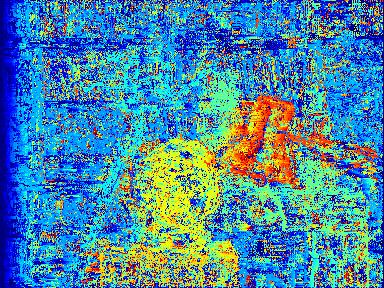
\includegraphics[height=20em]{prob2a}
  \caption{Disparity map from minimizing cost-volume without filtering}
  \label{fig:p2a}
\end{figure*}

\spart{b} To try to eliminate some of the noise, we build a bilateral kernel from the original image to try to preserve outlines of shapes, since we expect objects to have relatively constant disparity. We apply the bilateral kernel to the cost-volume to get the mapping in figure \ref{fig:p2b}. This method is far less noisy, but still is rather splotchy and loses a lot of the fine detail from the original mapping. This makes sense because bilateral filtering blurs details, while retaining edges.

\begin{figure*}[!h]
	\centering
	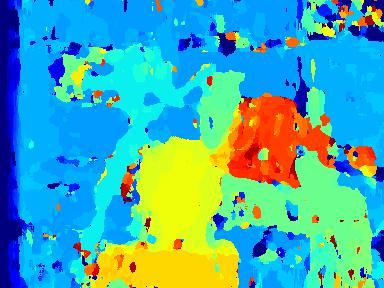
\includegraphics[height=20em]{prob2b}
	\caption{Disparity map from minimizing a bilaterally filtered cost-volume}
	\label{fig:p2b}
\end{figure*}


\solution{3} 

\spart{a} To implement the Viterbi forward-back algorithm, I used the fact that our smoothness cost function gave only four options for  $\arg\min$ of $d'$ for $\tilde{C}[x,d']+S(d,d')$ to build an options matrix with dimensions $H,D,4$ where $H$ is the height of the image, $D$ is the depth of the cost volume and 4 comes from the four options. Then, I found the argmin along its third axis to minimize every part of the problem for a given value of $x$ in parallel. Then I just assign $z[x,d] $ as the argmin, and $\bar{C}[x,d]$ as the element of the options matrix that gave the minimum plus $C[x,d]$. The result is shown in Figure \ref{fig:p3a}. There are a lot of streaking artifacts, because each horizontal line was separately minimized.

\begin{figure*}[!h]
	\centering
	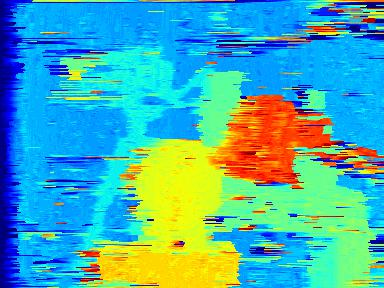
\includegraphics[height=19em]{prob3a}
	\caption{Disparity map from Viterbi left-right algorithm}
	\label{fig:p3a}
\end{figure*}

\spart{b} For this problem I implemented a similar algorithm in SGM. I used the same function to compute the augmented cost volumes as in part (a), without backtracking, just flipped and transposed along the $X,Y$ axes to find augmented cost volumes in left-right, right-left, up-down and down-up directions, then taking the argmin along the $D$ axis. There are less obvious streaking artifacts because the different directions help to smooth them out.

\begin{figure*}[!h]
	\centering
	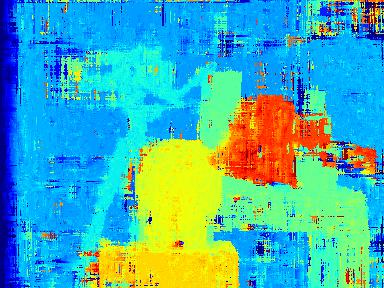
\includegraphics[height=19em]{prob3b}
	\caption{Disparity map from SGM}
	\label{fig:p3b}
\end{figure*}

\solution{4}

In this problem we compute an optical flow mapping of a pair of images from consecutive frames from a camera using the Lucas-Kanade Method. A key assumption to this method is that the two images were taken with only a short period of time between them, or that the velocity of objects is slow enough that pixels remain close to where they were located in the previous frame.

To do the computation, we compute a time gradient image, $I_t$, and $I_x,_yy$ gradient images for the average of the two frames. The time gradient is simply the second image's intensity subtracting the first image's intensity, and the $I_x,I_y$ gradients are computed using convolution of the average of the two frames' intensities. 
If we assume that the flow follows the following equation,
\begin{align}
	I_x \left[x',y'\right] u + I_y \left[x',y'\right] v = -I_t \left[x',y'\right]
\end{align}
then we can construct a quadratic minimization problem for $u,v$ to solve with least squares:
\begin{align}
	u(x,y), v(x,y) = \arg\min_{u,v} \sum_{(x',y')} \left(I_x \left[x',y'\right]u + I_y \left[x',y'\right] v + I_t \left[x',y'\right]\right)^2
\end{align}
If we take the derivatives in terms of $u,v$ and set them equal to 0, we get
\begin{align}
	\mathbf{0} = \begin{bmatrix}
		\sum_{(x',y')} 2\left(I_x^2 \left[x',y'\right] u + I_x \left[x',y'\right] I_y \left[x',y'\right] v + I_x \left[x',y'\right] I_t \left[x',y'\right]\right) \\
		\sum_{(x',y')} 2\left(I_x \left[x',y'\right] I_y \left[x',y'\right] u + I_y^2 \left[x',y'\right] v + I_y \left[x',y'\right] I_t \left[x',y'\right]\right)
	\end{bmatrix}
\end{align}
We can then formulate this as a matrix equation to solve in least squares,
\begin{align}
	\begin{bmatrix}
		\sum I_x^2 +\epsilon & \sum I_xI_y \\
		\sum I_xI_y & \sum I_y^2 + \epsilon
	\end{bmatrix} \begin{bmatrix}
	u \\ v
	\end{bmatrix} = - \begin{bmatrix}
	\sum I_xI_t \\ \sum I_yI_t
	\end{bmatrix}
\end{align}
where the sums are local summations of pixels in a range of $\pm W$ in the $x,y$ directions, and $\epsilon$ is a small number added to the diagonal elements to make inverting the matrix more stable. The local summations can be computed for each pixel in parallel using a convolution with a kernel of all ones. To make this solution possible with elementwise operations, we can then find the $2\times2$ inverse by hand to solve for $u,v$, 
\begin{align}
	 u = \dfrac{\left(\sum I_xI_y\right)\left(\sum I_y I_t\right) - \left(\sum I_y^2\right)\left(\sum I_x I_t\right)}{\left(\sum I_x^2\right)\left(\sum I_y^2\right)-\left(\sum I_xI_y\right)\left(\sum I_xI_y\right)} \\
	 v = \dfrac{\left(\sum I_xI_y\right)\left(\sum I_x I_t\right) - \left(\sum I_x^2\right)\left(\sum I_y I_t\right)}{\left(\sum I_x^2\right)\left(\sum I_y^2\right)-\left(\sum I_xI_y\right)\left(\sum I_xI_y\right)}
\end{align}
The result of the algorithm is shown in figure \ref{fig:p4}.
\begin{figure*}[!h]
	\centering
	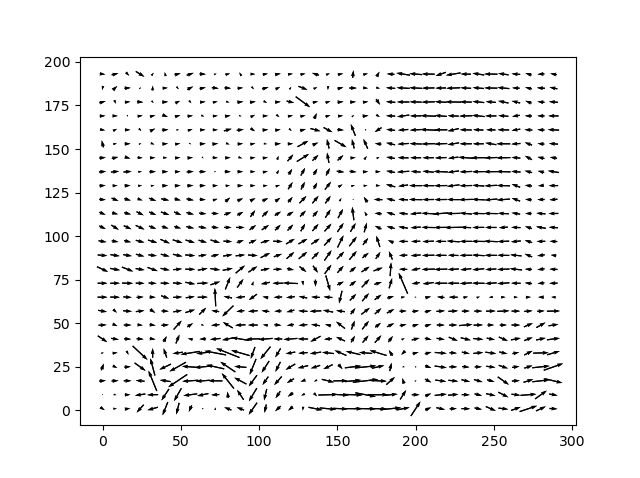
\includegraphics[height=35em]{prob4}
	\caption{Optical Flow using Lucas-Kanade Method}
	\label{fig:p4}
\end{figure*}


%%%%%%%%%% Important, you must edit and complete the informational
%%%%%%%%%% section below. If you discussed the problem set with no
%%%%%%%%%% one, edit it to say no discussions or external resources.
\info

This problem set took approximately 25 hours of effort (a very large part of which was dedicated to bugfixing when trying to parallelize problem 3a)

I discussed this problem set with no one.

% Note that you might have to escape some special symbols in URLS like \_
I also got hints from the following sources:
\begin{itemize}
	\item numpy.where documentation (p3a), \url{https://numpy.org/doc/stable/reference/generated/numpy.where.html}
	\item numpy.transpose documentation (p3b), \url{https://numpy.org/doc/stable/reference/generated/numpy.transpose.html}
\end{itemize}

\end{document}
